\section{Sequence Diagram}

\subsection{Sequence Diagram đăng nhập / đăng ký}
\begin{figure}[H]
    \centering
    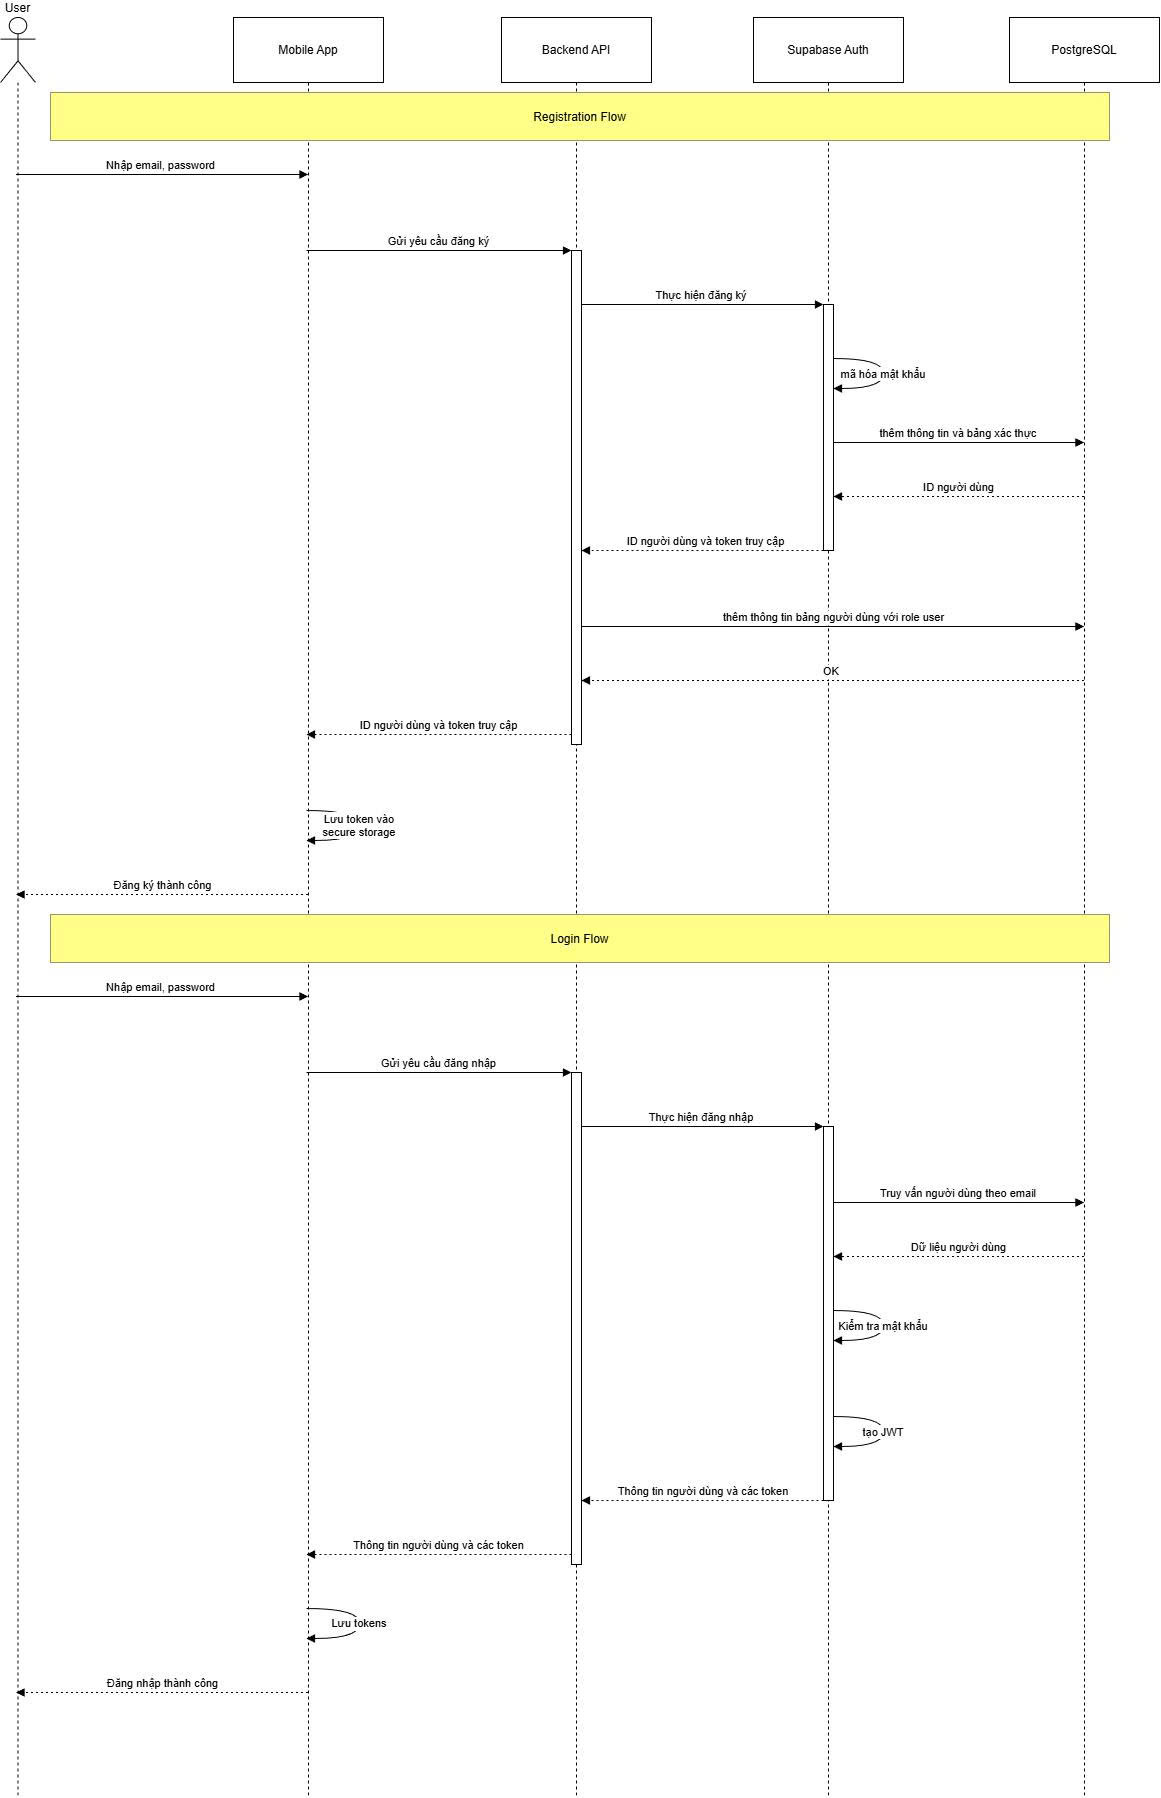
\includegraphics[width=0.7\textwidth]{figures/se_dndk.jpg}
    \caption{Sequence Diagram - Đăng nhập/Đăng ký}
    \label{fig:se_dndk}
\end{figure}

Sơ đồ mô tả quy trình đăng nhập và đăng ký người dùng trong hệ thống. 
Người dùng gửi thông tin xác thực thông qua ứng dụng, hệ thống kiểm tra dữ liệu với cơ sở dữ liệu Supabase. 
Trong trường hợp người dùng chưa tồn tại, hệ thống tiến hành tạo tài khoản mới và lưu trữ thông tin. 
Sau khi xác thực thành công, hệ thống khởi tạo phiên làm việc và trả kết quả cho người dùng.

%--------------------------------------------------

\subsection{Sequence Diagram đặt lịch}
\begin{figure}[H]
    \centering
    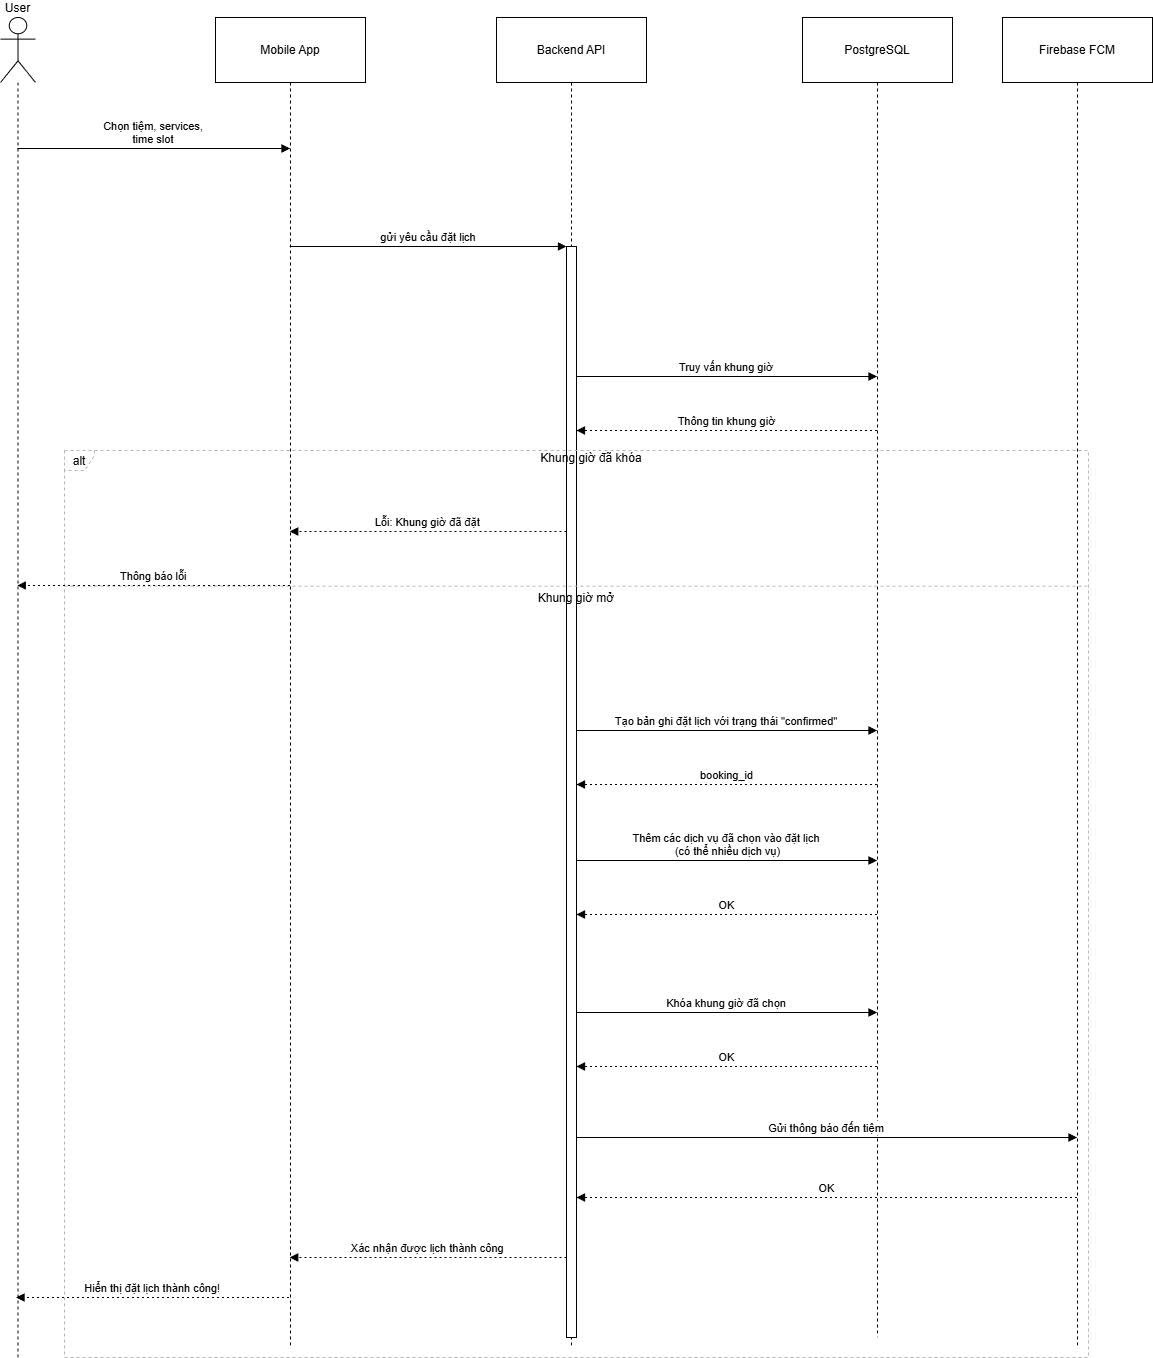
\includegraphics[width=0.8\textwidth]{figures/se_booking.jpg}
    \caption{Sequence Diagram - Đặt lịch}
    \label{fig:se_booking}
\end{figure}

Sơ đồ thể hiện quy trình đặt lịch dịch vụ của người dùng. 
Người dùng lựa chọn tiệm tóc, dịch vụ và khung giờ mong muốn, hệ thống kiểm tra tính khả dụng của thời gian trong cơ sở dữ liệu. 
Nếu hợp lệ, hệ thống tạo lịch hẹn và cập nhật trạng thái khung giờ tương ứng. 
Kết quả đặt lịch được phản hồi lại cho người dùng.

%--------------------------------------------------

\subsection{Sequence Diagram tạo tiệm tóc}
\begin{figure}[H]
    \centering
    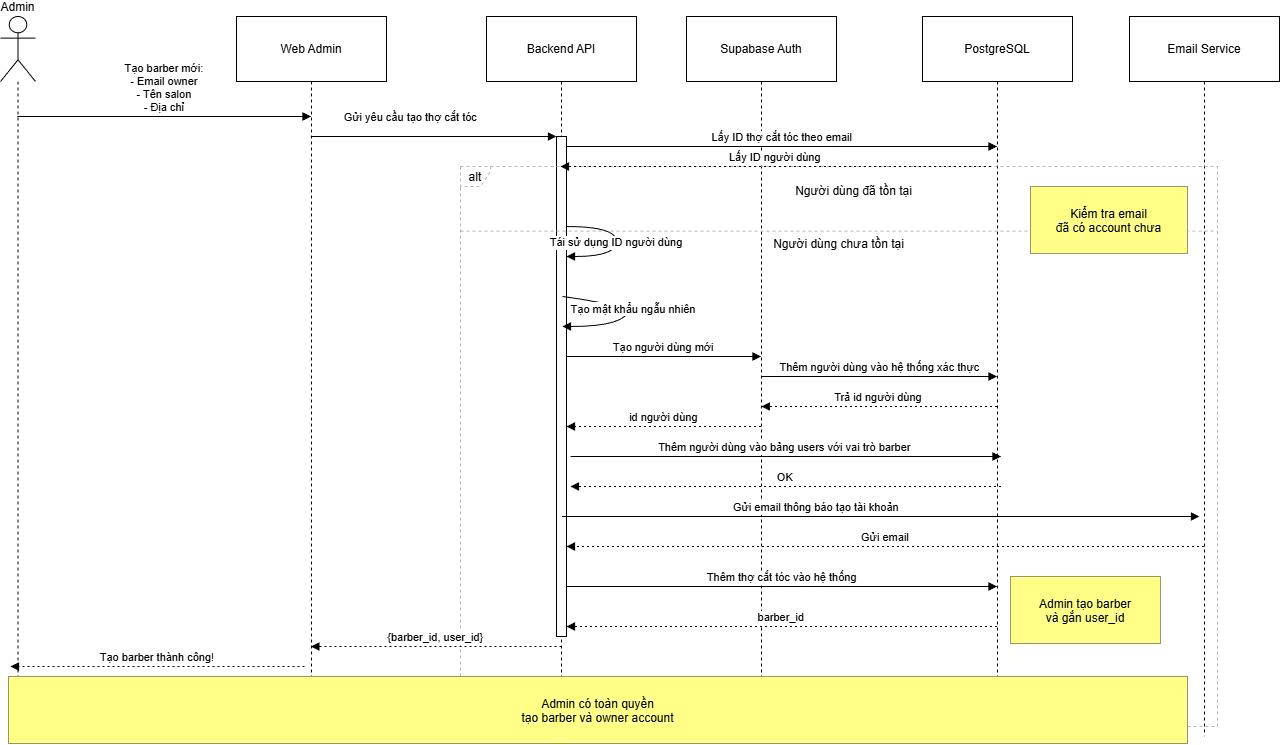
\includegraphics[width=0.7\textwidth]{figures/se_tao_barber.jpg}
    \caption{Sequence Diagram - Tạo tiệm tóc}
    \label{fig:se_tao_barber}
\end{figure}

Sơ đồ mô tả quá trình tạo mới tiệm tóc trong hệ thống. 
Chủ tiệm nhập thông tin tiệm thông qua giao diện ứng dụng, hệ thống tiến hành kiểm tra và lưu dữ liệu vào cơ sở dữ liệu Supabase. 
Sau khi tạo thành công, tiệm được kích hoạt để phục vụ các chức năng quản lý và đặt lịch.

%--------------------------------------------------

\subsection{Sequence Diagram quản lý dịch vụ tiệm tóc}
\begin{figure}[H]
    \centering
    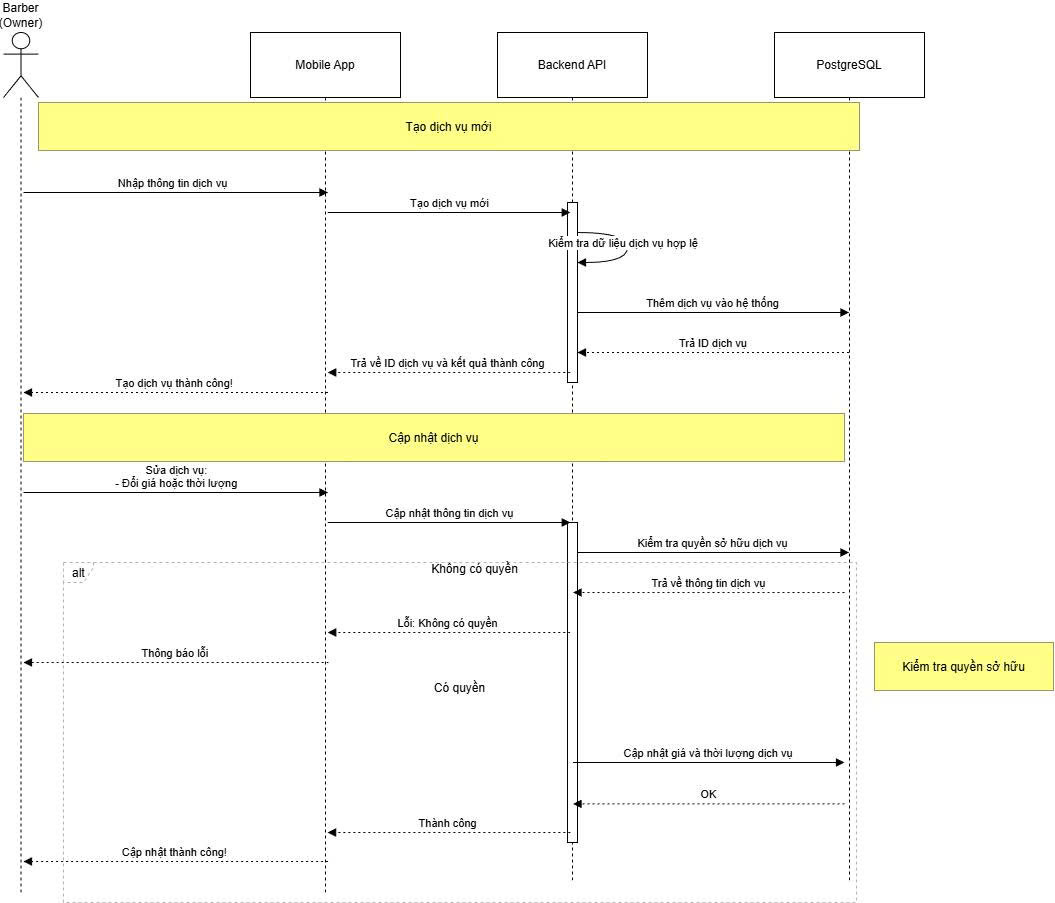
\includegraphics[width=1\textwidth]{figures/se_dv.jpg}
    \caption{Sequence Diagram - Quản lý dịch vụ}
    \label{fig:se_dv}
\end{figure}

Sơ đồ biểu diễn các thao tác quản lý dịch vụ của tiệm tóc bao gồm thêm, chỉnh sửa và xóa dịch vụ. 
Hệ thống tiếp nhận yêu cầu từ chủ tiệm, thực hiện cập nhật dữ liệu tương ứng trong cơ sở dữ liệu và phản hồi kết quả xử lý.

%--------------------------------------------------

\subsection{Sequence Diagram quản lý thời gian}
\begin{figure}[H]
    \centering
    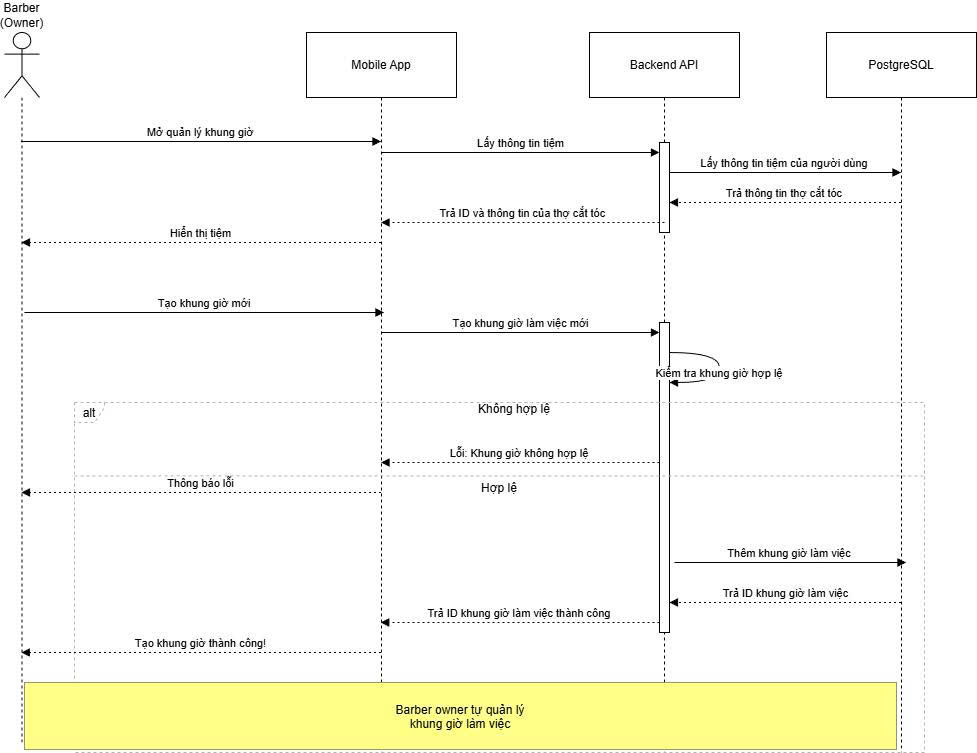
\includegraphics[width=1\textwidth]{figures/se_time_slot.jpg}
    \caption{Sequence Diagram - Quản lý thời gian}
    \label{fig:se_time_slot}
\end{figure}

Sơ đồ mô tả quy trình quản lý các khung giờ làm việc của tiệm tóc. 
Chủ tiệm thực hiện thiết lập hoặc điều chỉnh thời gian làm việc, hệ thống lưu trữ và đồng bộ dữ liệu với cơ sở dữ liệu. 
Các khung giờ này được sử dụng trong chức năng đặt lịch của người dùng.

%--------------------------------------------------

\subsection{Sequence Diagram cập nhật hồ sơ thợ cắt tóc}
\begin{figure}[H]
    \centering
    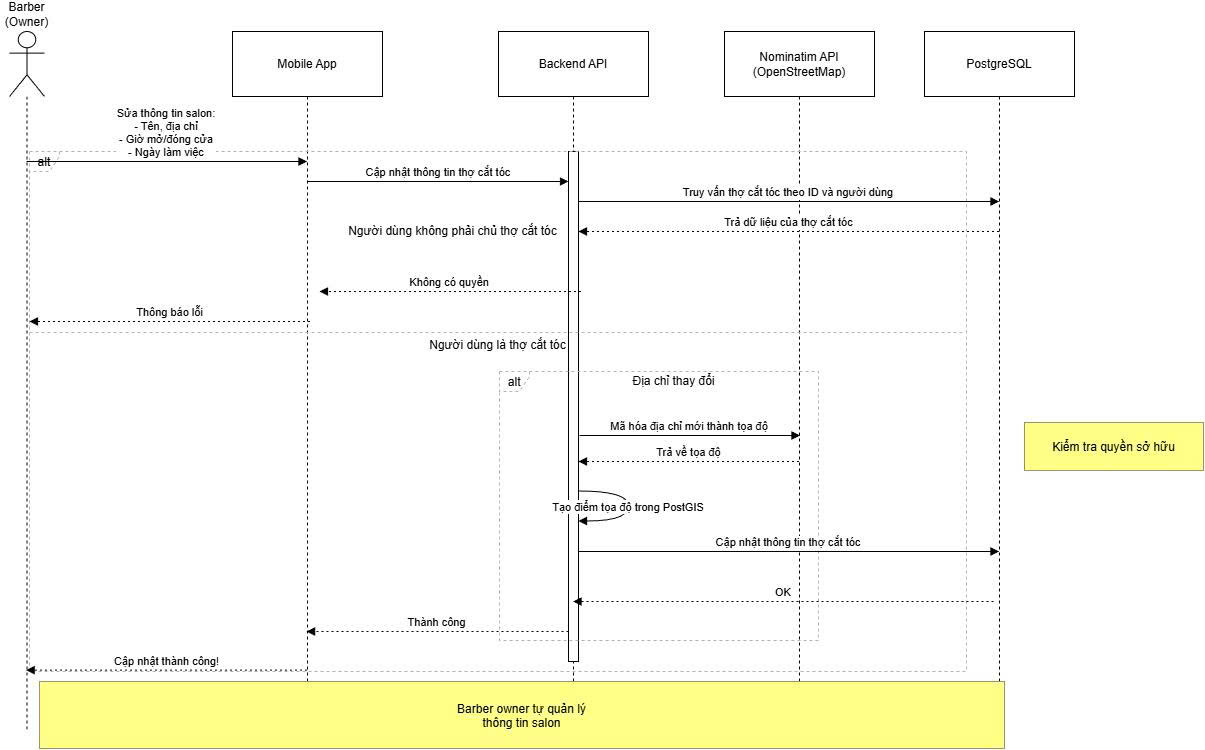
\includegraphics[width=1\textwidth]{figures/se_profile_tho.jpg}
    \caption{Sequence Diagram - Cập nhật hồ sơ thợ}
    \label{fig:se_profile_tho}
\end{figure}

Sơ đồ thể hiện quá trình cập nhật thông tin hồ sơ của thợ cắt tóc. 
Dữ liệu được chỉnh sửa thông qua giao diện ứng dụng và lưu trữ vào cơ sở dữ liệu sau khi kiểm tra hợp lệ. 

%--------------------------------------------------

\subsection{Sequence Diagram quản lý yêu cầu hợp tác}
\begin{figure}[H]
    \centering
    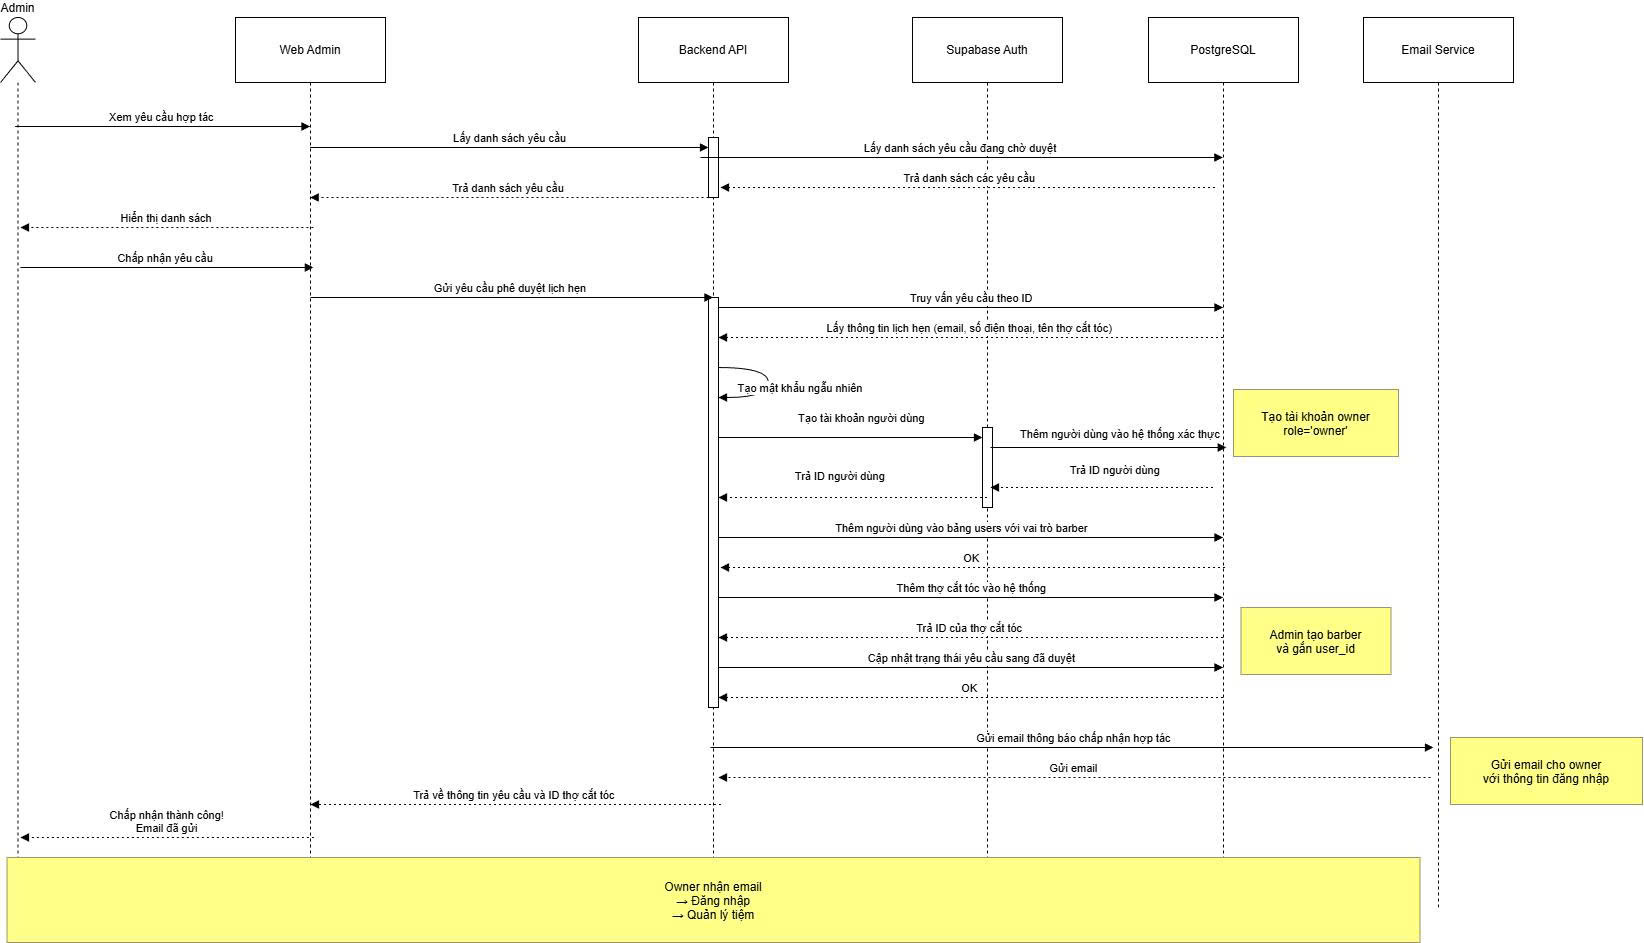
\includegraphics[width=1\textwidth]{figures/se_yeu_cau.jpg}
    \caption{Sequence Diagram - Quản lý yêu cầu hợp tác}
    \label{fig:se_yeu_cau}
\end{figure}

Sơ đồ mô tả quy trình xử lý các yêu cầu hợp tác. 
Hệ thống tiếp nhận yêu cầu, lưu trữ trạng thái và cho phép chủ tiệm phê duyệt hoặc từ chối yêu cầu hợp tác.

%--------------------------------------------------

\subsection{Sequence Diagram gợi ý kiểu tóc}
\begin{figure}[H]
    \centering
    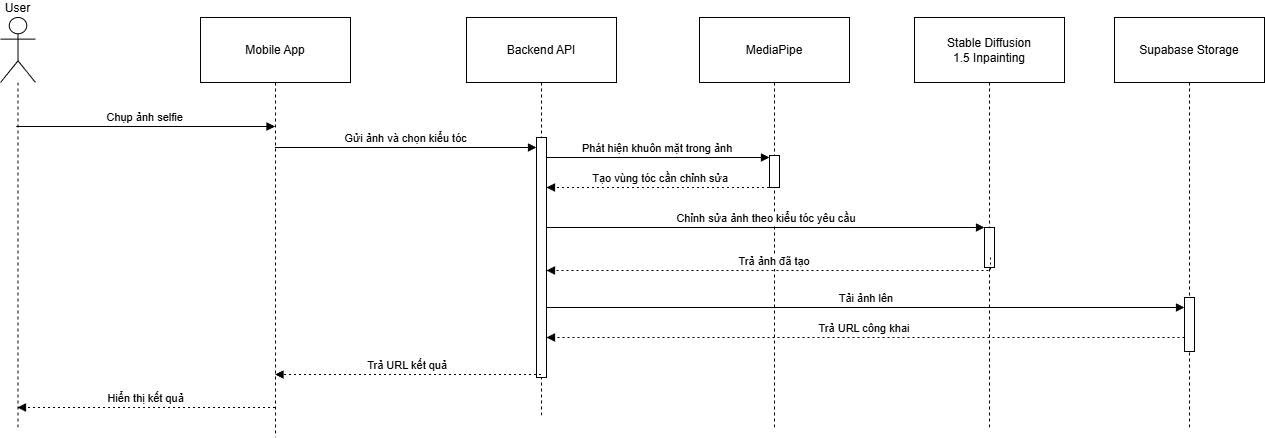
\includegraphics[width=1\textwidth]{figures/se_toc.jpg}
    \caption{Sequence Diagram - Gợi ý kiểu tóc}
    \label{fig:se_toc}
\end{figure}

Sơ đồ thể hiện quá trình hệ thống AI gợi ý kiểu tóc cho người dùng. 
Dữ liệu đầu vào từ người dùng được gửi đến mô hình AI, hệ thống sinh ra kết quả gợi ý phù hợp và phản hồi cho người dùng.

%--------------------------------------------------

\subsection{Sequence Diagram chăm sóc da mặt}
\begin{figure}[H]
    \centering
    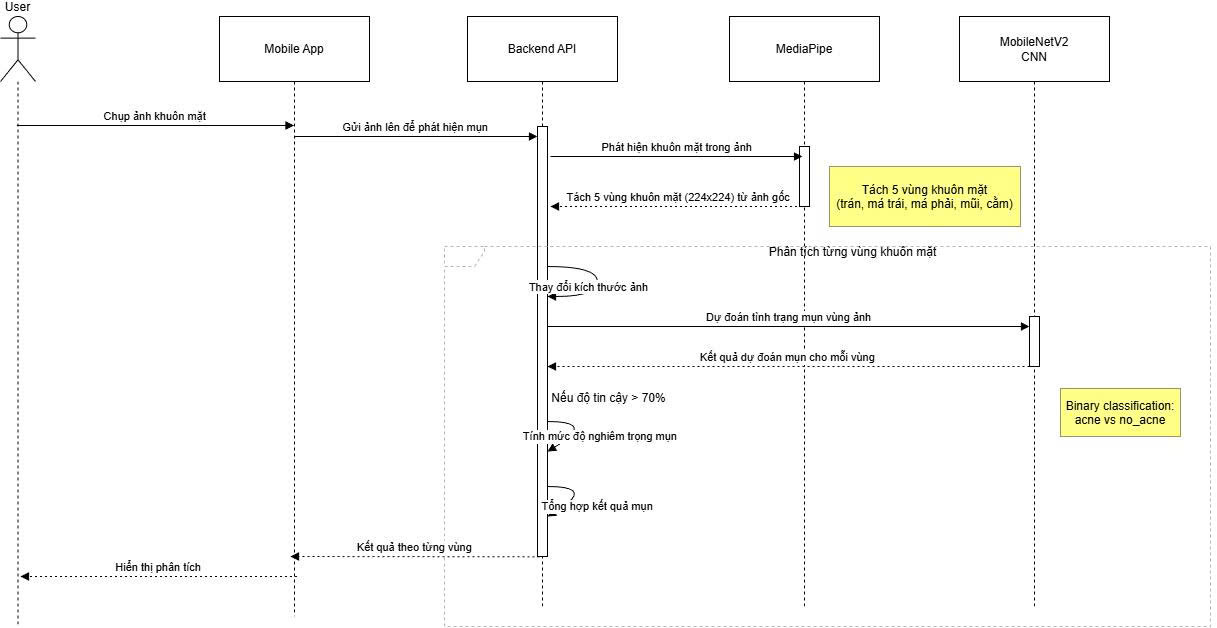
\includegraphics[width=1\textwidth]{figures/se_mun.jpg}
    \caption{Sequence Diagram - Chăm sóc da mặt}
    \label{fig:se_mun}
\end{figure}

Sơ đồ mô tả quy trình tư vấn chăm sóc da mặt dựa trên AI. 
Hệ thống tiếp nhận thông tin hoặc hình ảnh từ người dùng, xử lý bằng mô hình AI và kết hợp dữ liệu để đưa ra khuyến nghị phù hợp.

%--------------------------------------------------

\subsection{Sequence Diagram chat với AI}
\begin{figure}[H]
    \centering
    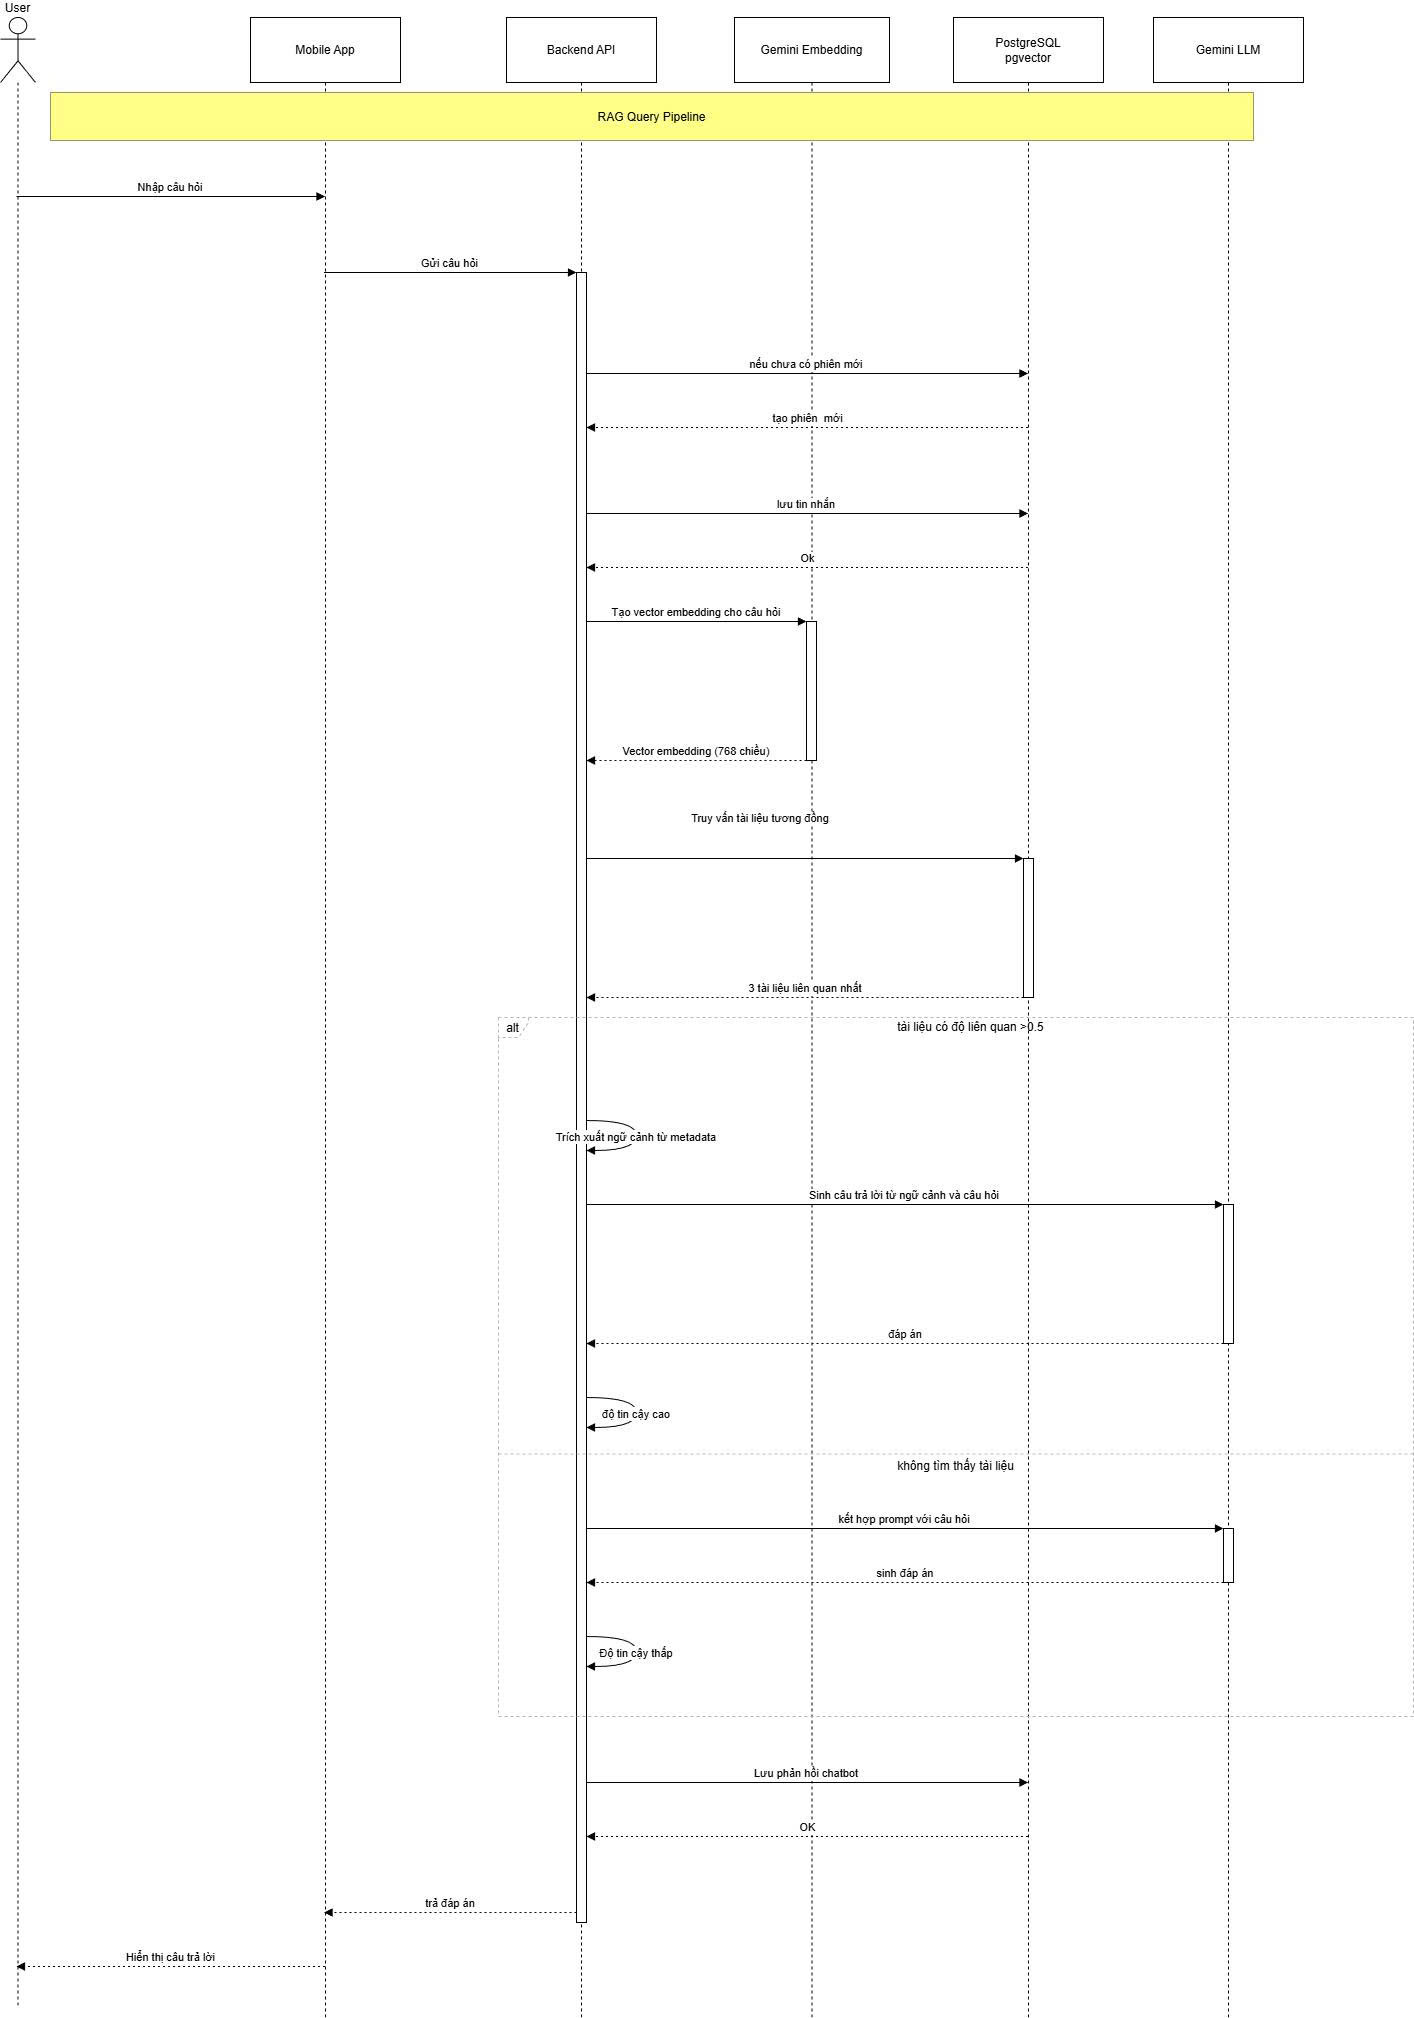
\includegraphics[width=0.8\textwidth]{figures/se_chat.jpg}
    \caption{Sequence Diagram - Chat với AI}
    \label{fig:se_chat}
\end{figure}

Sơ đồ mô tả chi tiết quá trình tương tác giữa mô hình AI và cơ sở dữ liệu private trong kiến trúc Retrieval-Augmented Generation (RAG) của hệ thống BarberGo.

Khi người dùng gửi câu hỏi thông qua ứng dụng di động, hệ thống backend sẽ ghi nhận nội dung câu hỏi và tiến hành chuyển đổi câu hỏi thành vector embedding bằng mô hình embedding. Vector này sau đó được sử dụng để truy vấn cơ sở dữ liệu vector (pgvector trên PostgreSQL), nơi lưu trữ các tài liệu private của hệ thống như thông tin dịch vụ, kiến thức chăm sóc tóc và quy trình nghiệp vụ.

Kết quả truy vấn là tập các tài liệu có độ tương đồng cao nhất với câu hỏi của người dùng. Các tài liệu này được trích xuất nội dung và đóng vai trò là ngữ cảnh (context), sau đó được kết hợp cùng câu hỏi ban đầu để gửi đến mô hình LLM.

Nhờ việc bổ sung ngữ cảnh từ dữ liệu private, mô hình LLM không chỉ dựa vào kiến thức chung đã được huấn luyện trước mà còn tạo sinh câu trả lời dựa trên dữ liệu thực tế của hệ thống. Cách tiếp cận này giúp giảm hiện tượng hallucination, tăng tính chính xác và đảm bảo câu trả lời phù hợp với bối cảnh nghiệp vụ của BarberGo.

\subsection{Sequence Diagram quản lý Prompt Knowledge Base}
\begin{figure}[H]
    \centering
    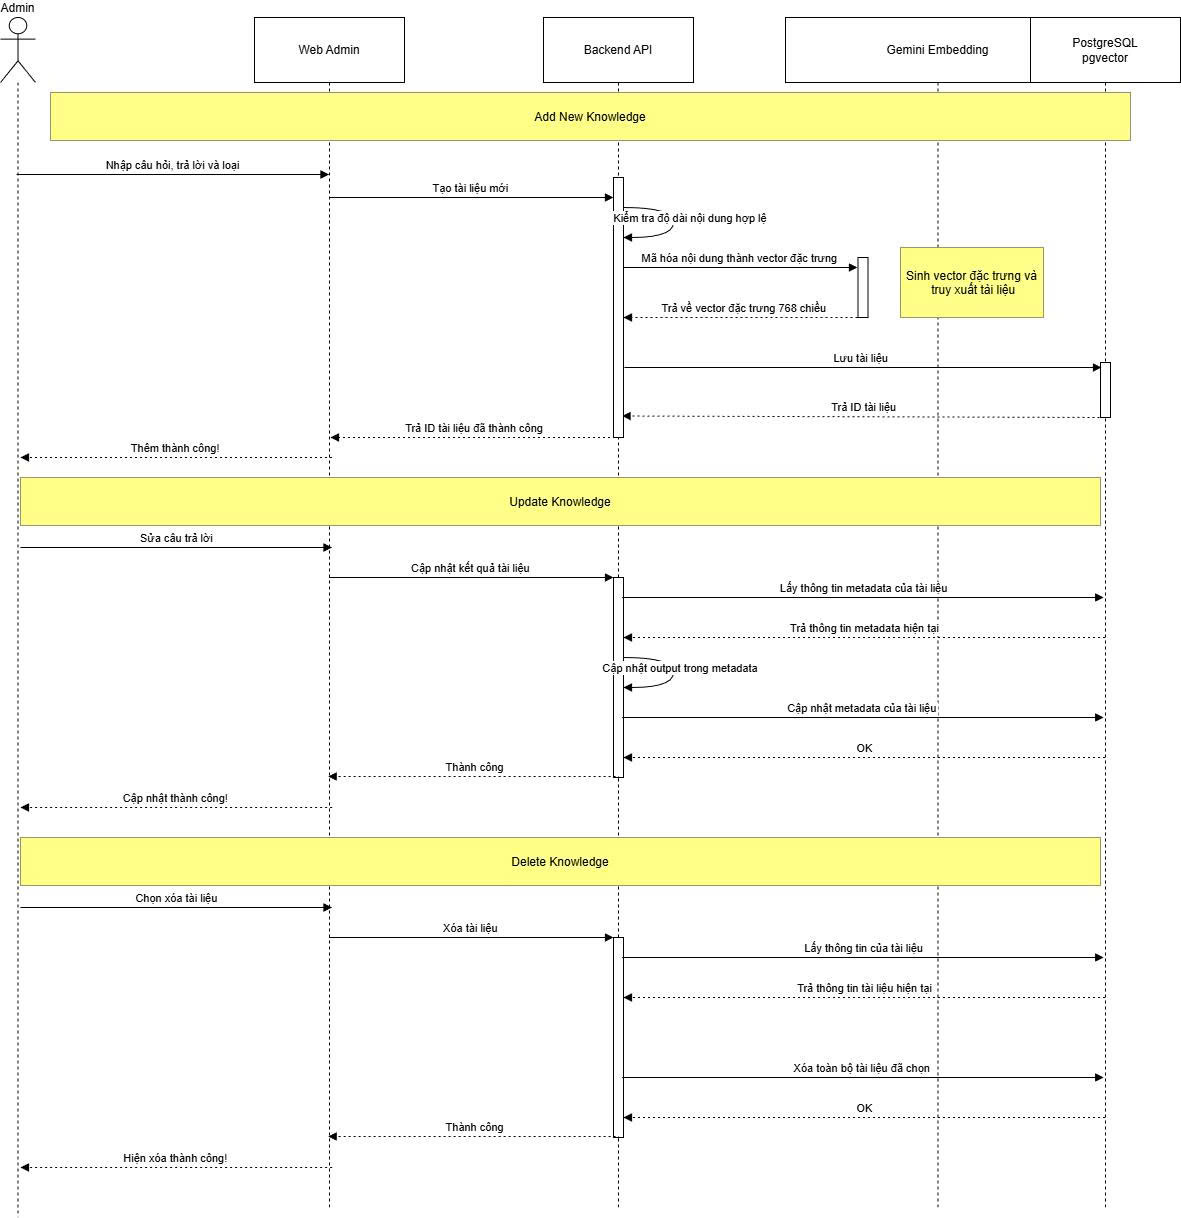
\includegraphics[width=1\textwidth]{figures/se_promy.jpg}
    \caption{Sequence Diagram - Quản lý Prompt Knowledge Base}
    \label{fig:se_promy}
\end{figure}

Sơ đồ mô tả quá trình quản lý kho tri thức phục vụ cho hệ thống AI. 
Quản trị viên thực hiện thêm, chỉnh sửa hoặc xóa nội dung dữ liệu tri thức. 
Hệ thống cập nhật thông tin vào cơ sở dữ liệu và vector database để phục vụ cơ chế RAG.

%--------------------------------------------------

\subsection{Sequence Diagram gắn định vị}
\begin{figure}[H]
    \centering
    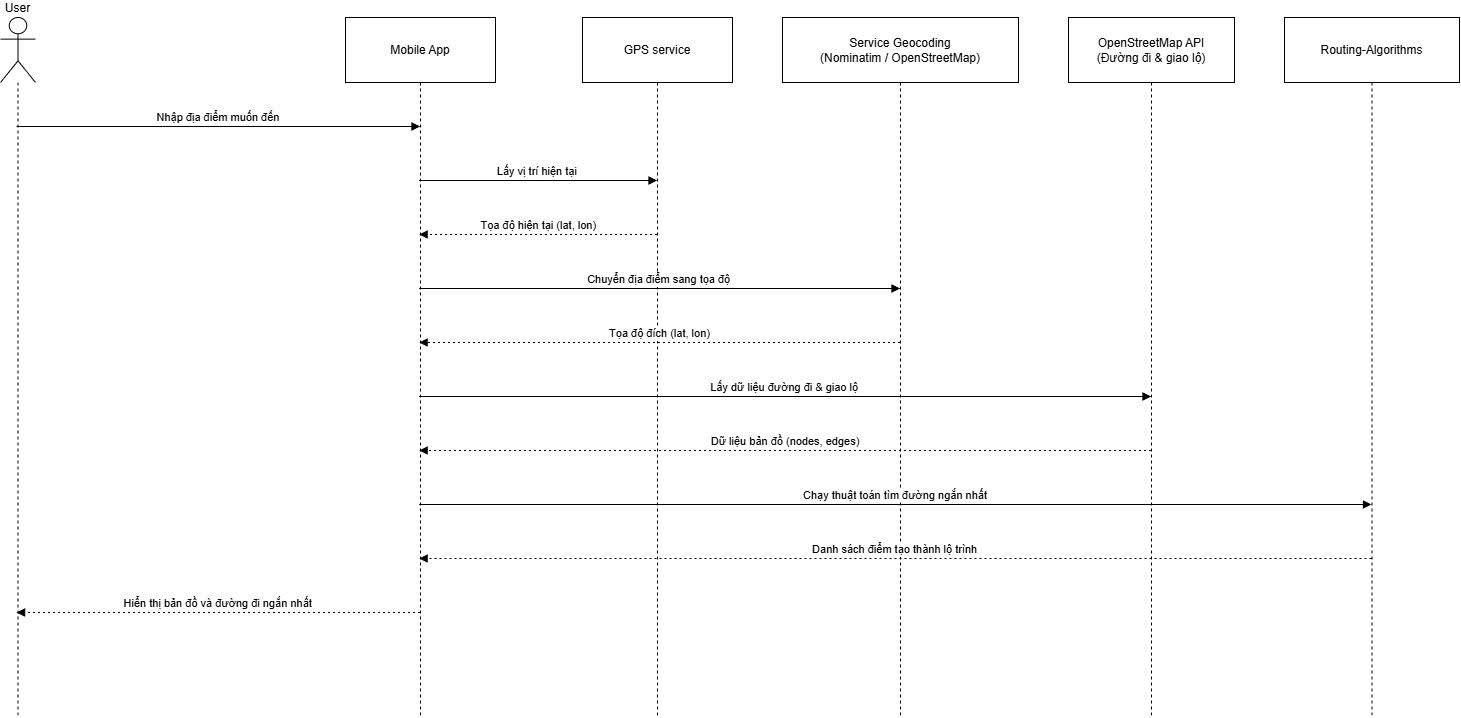
\includegraphics[width=1\textwidth]{figures/se_map.jpg}
    \caption{Sequence Diagram - Gắn định vị}
    \label{fig:se_map}
\end{figure}

Sơ đồ thể hiện quy trình gắn định vị cho tiệm tóc. 
Khi người dùng chọn địa chỉ tiệm, hệ thống truy vấn dữ liệu kinh độ và vĩ độ từ cơ sở dữ liệu Supabase. 
Dựa trên dữ liệu này, hệ thống thực hiện tìm kiếm và vẽ lộ trình di chuyển trên bản đồ nhằm hỗ trợ người dùng đến tiệm một cách thuận tiện.
